\subsection{Experiment 2: Expanding Experiment 1 to use all four arithmetic operations} \label{sec:experiment-2}

\subsubsection{Objective}

The goal of this experiment is similar to Experiment 1 where we attempted to verify that the presence of symbols while training an artificial neural network results in significant increases in the network accuracy. Experiment 1 used only the addition operation. This experiment expands the dataset used to include all four arithmetic operations.

\subsubsection{Method}

For this experiment we use the \textbf{Noisy Inputs with Intermediate Classification (NC)} from the previous experiment as the model that is trained in the presence of symbols. Figure \ref{fig:sequential-model-symbols-noisy-times} depicts the NC model learning to do multiplication. \textbf{The Noisy Inputs Only (NO)} model is also used for comparison as the model trained without symbols. NO is slightly modified to provide output on its intermediate time steps. The output provided during training for these intermediate time steps is a vector with all its features set to a dummy value of 0.5 to signify that no symbol is provided. Figure \ref{fig:sequential-model-noisy-only-divide} shows an example of the NO model performing division.

The dataset used for Experiment 1 is expanded to include four different arithmetic operations (addition, subtraction, multiplication and division). For each operation, single digit inputs from the range of 0 to 9 are used to form combinations of operands and for each combination, ten MNIST examples are sampled. For both addition and multiplication, all 100 combinations are included in the dataset. However, for subtraction and division the combinations are selected so that for subtraction, no combinations that would result in negative outputs would be included and for division, division by zero is avoided. K-fold cross-validation is used, with k set to 5, to split the samples of each combination into a training, validation and test set. The training and testing of each model is repeated five times and the accuracy obtained on the test set is recorded for each attempt. Just like in Experiment 1, all combinations of digits are provided for training.

\begin{figure}[t]
	\centering
	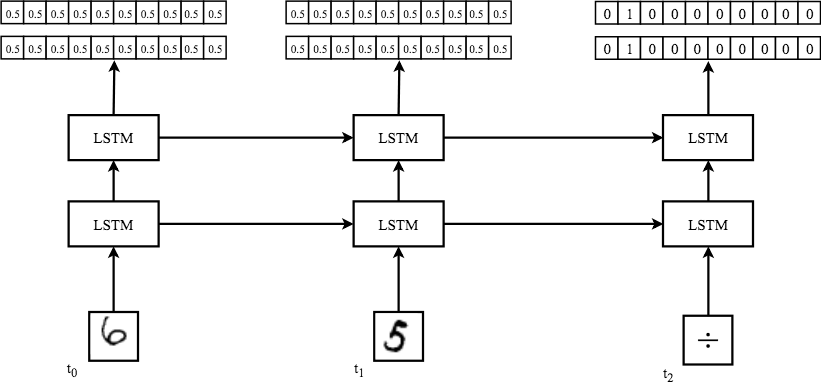
\includegraphics[max width=\textwidth]{sequential-model-noisy-only-divide}
	\caption{The Noisy Inputs Only (NO). A deep LSTM network that accepts a sequence of two operands and an operator modeling the operation: 6 / 5. Only noisy operands are provided. The output represents the quotient and the remainder, which are both 1.}
	\label{fig:sequential-model-noisy-only-divide}
\end{figure}

Both models have the same architectures used in Experiment 1. The models accept a sequence of three 28x28 images. The first two images are of the handwritten digits representing the operands of the operation. The third image is that of the operator. The models output two one-hot vectors representing the least and most significant values of the output at each time step. When each of the operands is presented, the network attempts to output the correct signals on the one-hot vector outputs representing the value of the digit presented on the input. When finally the operator is presented, the network is trained to perform the operation and output the result. Both models use two hidden LSTM layers each with 512 units.

\begin{figure}[t]
	\centering
	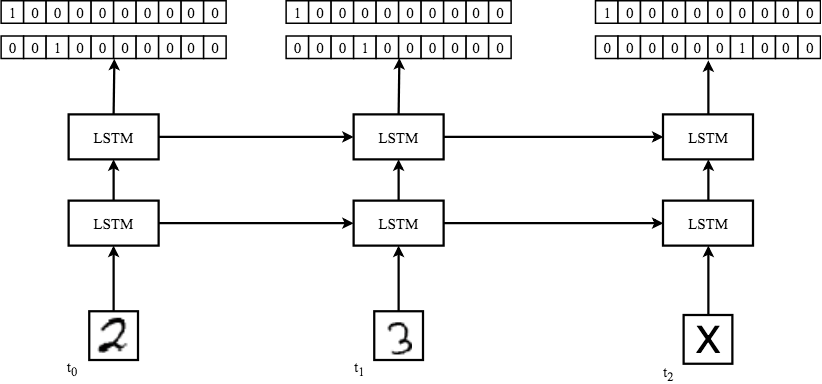
\includegraphics[max width=\textwidth]{sequential-model-symbols-noisy-times}
	\caption{Noisy Inputs with Intermediate Classification (NC). A deep LSTM network that accepts a sequence of two operands and an operator modeling the operation 2 x 3. Both the noisy operands and their corresponding symbolic information are provided alongside one another.}
	\label{fig:sequential-model-symbols-noisy-times}
\end{figure}

\subsubsection{Results}

\begin{table}[p]
	\center
	\caption{A comparison of the mean accuracy and standard deviation of the models trained with and without classification on all four arithmetic operations. Also shown is the p-value of a hypothesis t-Test when compared to the NO method.}
	\label{tab:experiment-2-results-table}
	\begin{tabular}{ |c|c|c|c| } 
		\hline
		Method & Accuracy (\%) & Standard Deviation  & p-value, t-Test with NO Method\\ 
		NO & 60.75 & 0.02 & NA \\  
		NC & 77.36 & 0.03 & 0.00092\\  
		\hline
	\end{tabular}
\end{table}

\begin{figure}[p]
	\centering
	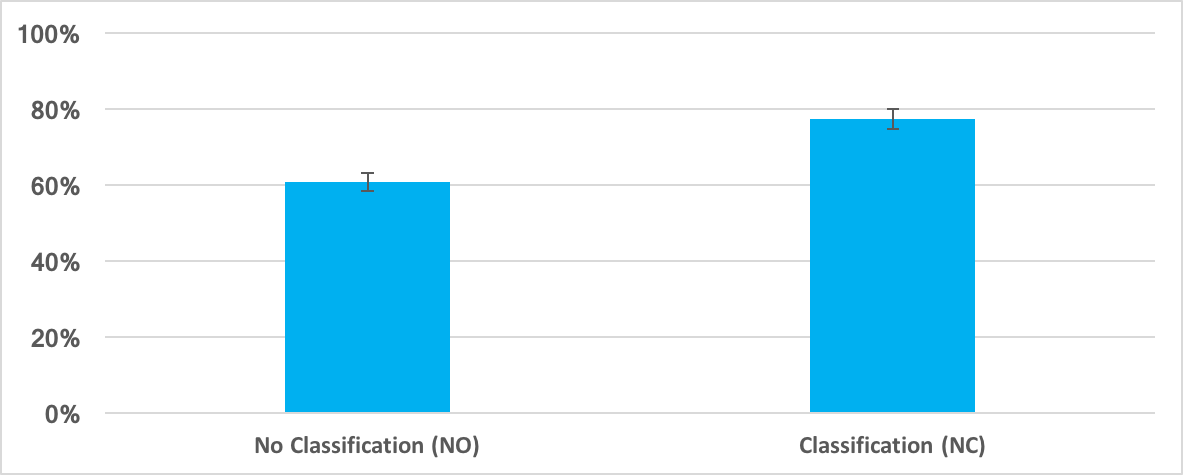
\includegraphics[max width=\textwidth]{experiment-2-results-chart}
	\caption{A comparison of the mean accuracy and 95\% confidence intervals of the models trained with and without classification on all four arithmetic operations.}
	\label{fig:experiment-2-results-chart}
\end{figure}

\begin{table}
	\center
	\caption{The mean accuracies of each arithmetic operation when tested on both the NO and NC models.}
	\label{tab:experiment-2-operations-table}
	\begin{tabular}{ |c|c|c|c|c| } 
		\hline
		Method & Addition (\%) & Subtraction (\%)  & Multiplication (\%) & Division (\%)\\ 
		NO & 63.35 & 60.77 & 61.4 & 57.48\\  
		NC & 78.5 & 77.71 & 80.23 & 73.0\\  
		\hline
	\end{tabular}
\end{table}

\begin{figure}[t]
	\centering
	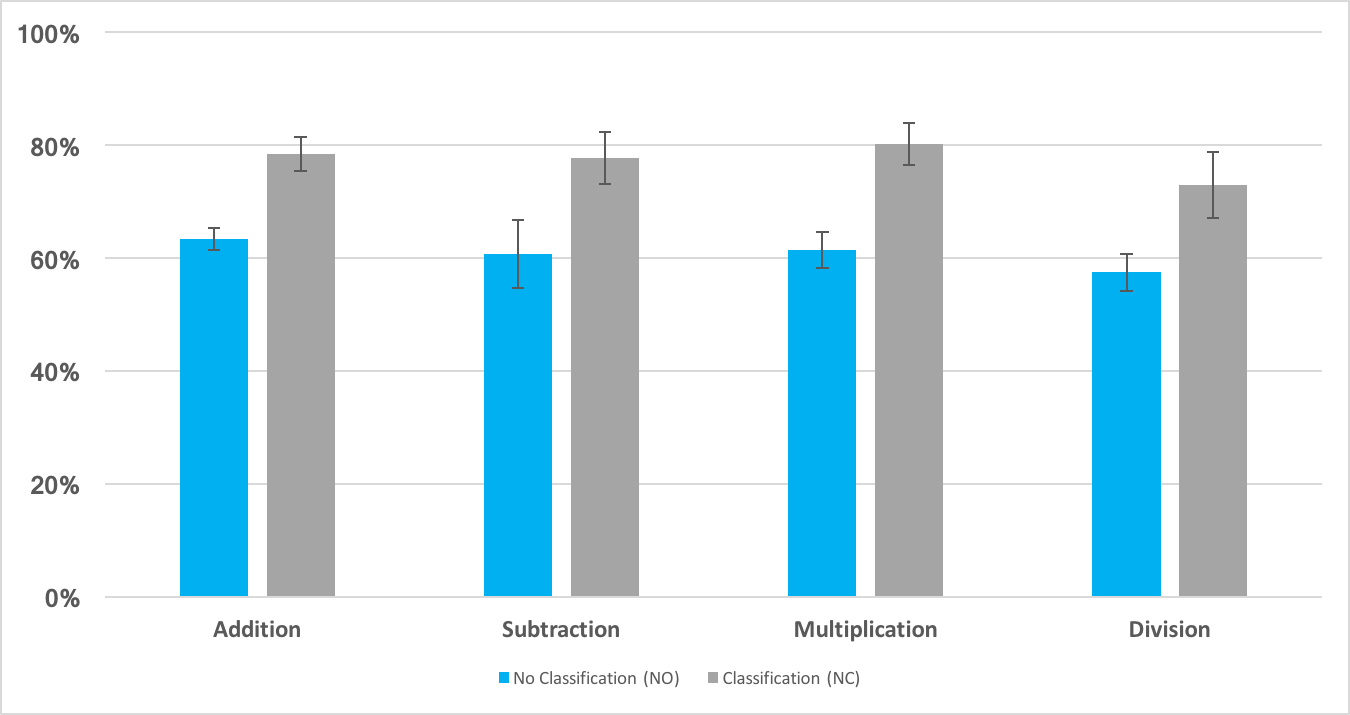
\includegraphics[max width=\textwidth]{experiment-2-operations-chart}
	\caption{A comparison of the mean accuracy and 95\% confidence intervals of each arithmetic operation on both models trained with and without classification.}
	\label{fig:experiment-2-operations-chart}
\end{figure}

Table \ref{tab:experiment-2-results-table} and Figure \ref{fig:experiment-2-results-chart} compare the results of the model trained without symbols (NO) with the model trained with symbols (NC). The model trained in the presence of symbols performs significantly better than the one trained without symbols. Table \ref{tab:experiment-2-operations-table} and Figure \ref{fig:experiment-2-operations-chart} show the accuracies obtained using each of these models when tested on each arithmetic operator independently.

\subsubsection{Discussion}

This experiment shows that the LSTM recurrent neural networks are capable of learning various types of arithmetic operations on images of handwritten digits and that the presence of symbolic knowledge during training significantly improves the accuracy of these models. With the exception of division, Table \ref{tab:experiment-2-operations-table} and Figure \ref{fig:experiment-2-operations-chart} show that when analyzing the accuracies of the models on each operator independently, we see that the mean accuracies are close to one another and close to the overall mean accuracy of the models. Division is a more complicated operation that involves finding a quotient and a remainder which could account of the reduced performance.